\chapter{Lagrangedichten, Felder und lokale Teilchenprozesse}

Bosonenfelder, Fermionenfelder und das elektromagnetische Feld erfüllen wellenartige Gleichungen. Diese Gleichungen enthalten die Felder selbst sowie ihre räumlichen und zeitlichen Ableitungen. Man könnte für jedes Feld eine eigene Bewegungsgleichung angeben; eine Lagrangedichte fasst jedoch das gesamte System in einem kompakten Ausdruck zusammen. Wendet man auf diesen Ausdruck die Euler--Lagrange-Regel an, erhält man gleichzeitig die Gleichungen für alle Felder.

Diese Konstruktion hängt eng mit dem Prinzip der stationären Wirkung zusammen. Hier geht es zunächst um eine konkretere Aufgabe: herauszufinden, wovon eine Feld-Lagrangedichte abhängt, mit ihr einige klassische Gleichungen herzuleiten und dieselben Feldausdrücke anschließend quantenmechanisch neu zu deuten. In der Quantentheorie bestimmt die Lagrangedichte die Bewegung und Wechselwirkung von Teilchen und letztlich die Amplituden und Wirkungsquerschnitte bei Stößen.

\section{Ein kompakter Formalismus für Feldgleichungen}

Für ein einzelnes Skalarfeld hängt die Lagrangedichte vom Feld und seinen ersten Ableitungen ab,
\begin{equation}
\mathcal L
=
\mathcal L\!\left(\phi,\partial_t\phi,\partial_x\phi,\ldots\right)
=
\mathcal L\!\left(\phi,\partial_\mu\phi\right).
\end{equation}
Bei Rechnungen ist die explizite Auflistung der zeitlichen und räumlichen Ableitungen oft hilfreicher; die Schreibweise \(\partial_\mu\phi\) fasst dieselbe Liste relativistisch zusammen.

\begin{figure}[htbp]
\centering
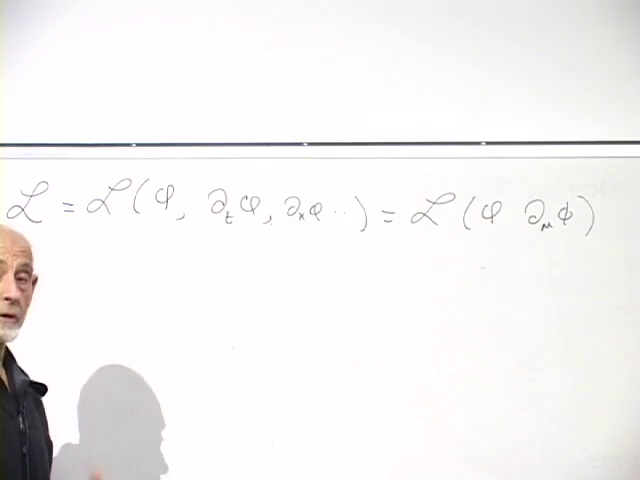
\includegraphics[width=0.82\textwidth]{lecture_09_figure_03.png}
\caption{Abhängigkeit einer Skalarfeld-Lagrangedichte vom Feld und seinen Raumzeit-Ableitungen.}
\lectureframe{00:03:56}
\end{figure}

Die Euler--Lagrange-Gleichung für Felder lautet
\begin{equation}
\frac{\partial}{\partial t}
\frac{\partial\mathcal L}{\partial\dot\phi}
+
\frac{\partial}{\partial x}
\frac{\partial\mathcal L}{\partial\phi_x}
+
\frac{\partial}{\partial y}
\frac{\partial\mathcal L}{\partial\phi_y}
+
\frac{\partial}{\partial z}
\frac{\partial\mathcal L}{\partial\phi_z}
=
\frac{\partial\mathcal L}{\partial\phi},
\end{equation}
wobei
\begin{equation}
\dot\phi=\frac{\partial\phi}{\partial t},
\qquad
\phi_x=\frac{\partial\phi}{\partial x},
\qquad
\phi_y=\frac{\partial\phi}{\partial y},
\qquad
\phi_z=\frac{\partial\phi}{\partial z}.
\end{equation}
Wenn \(\mathcal L\) mehrere Felder enthält, wird diese Regel für jedes Feld einzeln angewendet. Das Ergebnis ist das System der Bewegungsgleichungen.

Das einfachste Beispiel für ein Skalarfeld ist
\begin{equation}
\begin{split}
\mathcal L
&=
\frac12\dot\phi^2
-\frac12\phi_x^2
-\frac12\phi_y^2
-\frac12\phi_z^2
-V(\phi)
\\
&=
\frac12\dot\phi^2-\frac12(\boldsymbol\nabla\phi)^2-V(\phi).
\end{split}
\end{equation}
Die Terme mit räumlichen Ableitungen haben das entgegengesetzte Vorzeichen wie der Term mit der zeitlichen Ableitung. Leitet man die einzelnen Terme ab, erhält man
\begin{align}
\frac{\partial\mathcal L}{\partial\dot\phi}&=\dot\phi,
&
\frac{\partial\mathcal L}{\partial\phi_i}&=-\phi_i,
&
\frac{\partial\mathcal L}{\partial\phi}&=-V'(\phi),
\end{align}
und damit
\begin{equation}
\ddot\phi-\nabla^2\phi=-V'(\phi).
\end{equation}

\begin{figure}[htbp]
\centering
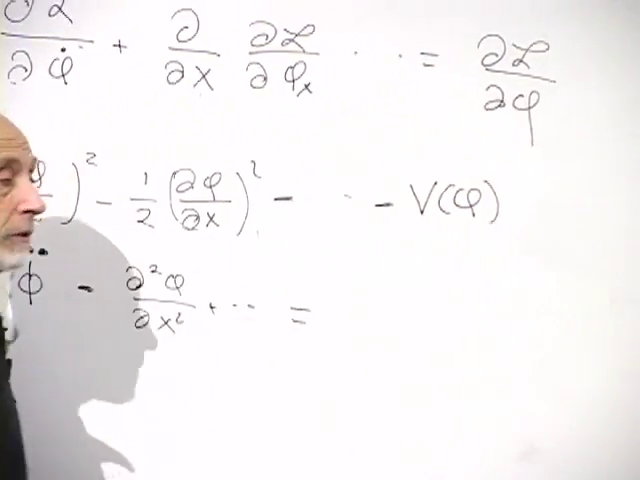
\includegraphics[width=0.74\textwidth]{lecture_09_figure_04.png}
\caption{Euler--Lagrange-Gleichung, Skalarfeld-Lagrangedichte und die von \(V(\phi)\) erzeugte Feldgleichung.}
\lectureframe{00:08:23}
\end{figure}

Dies ist die von der Skalarfeld-Lagrangedichte erzeugte Gleichung.\editorialnote{Der erhaltene Bildausschnitt ist am linken Rand abgeschnitten; die gezeigte Ergänzung ergibt sich eindeutig aus der unmittelbar vorausgehenden und anschließenden Herleitung.}

Hier ist \(V(\phi)\) die potenzielle Energiedichte des Feldes. Ein konstanter Beitrag zu \(V\) hat keinen Einfluss auf diese Gleichung, weil seine Ableitung verschwindet. Ein lineares Potential ist algebraisch möglich, hat aber keine untere Schranke: Die Feldenergie kann gegen minus unendlich gehen. Das erste stabile Beispiel ist daher
\begin{equation}
V(\phi)=\frac12m^2\phi^2,
\qquad
V'(\phi)=m^2\phi,
\end{equation}
woraus folgt
\begin{equation}
\ddot\phi-\nabla^2\phi=-m^2\phi.
\end{equation}

Um die Bedeutung von \(m\) sichtbar zu machen, setzen wir eine ebene Welle ein:
\begin{equation}
\phi(\mathbf x,t)=\phi_0e^{i\omega t-i\mathbf k\cdot\mathbf x}.
\end{equation}
Dann gilt
\begin{equation}
\ddot\phi=-\omega^2\phi,
\qquad
\nabla^2\phi=-\mathbf k^2\phi,
\end{equation}
sodass die Wellengleichung zu
\begin{equation}
-\omega^2\phi+\mathbf k^2\phi=-m^2\phi.
\end{equation}
wird. Nach dem Kürzen von \(\phi\) gilt
\begin{equation}
\omega^2=\mathbf k^2+m^2.
\end{equation}
In Einheiten mit \(\hbar=c=1\) sind Frequenz und Energie sowie Wellenzahl und Impuls gleich. Somit gilt
\begin{equation}
E^2=\mathbf p^2+m^2,
\end{equation}
oder, mit wieder eingesetzten Potenzen von \(c\), \(E^2=\mathbf p^2c^2+m^2c^4\). Der Parameter \(m\) ist die Masse eines Quants des Feldes.

Lorentz-Invarianz lässt sich bereits auf der Ebene des kompakten Ausdrucks sicherstellen. Ist \(\mathcal L\) ein Lorentz-Skalar, so sind seine Bewegungsgleichungen Lorentz-invariant. Das relative Vorzeichen zwischen zeitlichen und räumlichen Ableitungen entspricht dem vertrauten Raumzeit-Vorzeichen der speziellen Relativitätstheorie.

\section{Nichtlinearität und gekoppelte klassische Felder}

Höhere Potenzen eines Feldes führen zu einer neuen Art von Verhalten. Ist
\begin{equation}
V(\phi)=\frac12m^2\phi^2+g\phi^3,
\end{equation}
so gilt
\begin{equation}
\ddot\phi-\nabla^2\phi=-m^2\phi-3g\phi^2.
\end{equation}
Quadratische Terme in der Lagrangedichte ergeben lineare Gleichungen für das Feld. Kubische und höhere Terme führen zu nichtlinearen Gleichungen.

Der Unterschied zeigt sich in der Bewegung von Wellenpaketen. Bei einer linearen Gleichung lassen sich ein nach rechts und ein nach links laufendes Wellenpaket addieren, sodass eine weitere Lösung entsteht. Die Pakete überlagern sich eine Zeit lang und interferieren, durchdringen einander dann und laufen in ihrer ursprünglichen Form weiter. Bei nichtlinearen Termen beeinflussen sich die Pakete gegenseitig. Sie können gestreut oder verformt werden oder in kompliziertere Wellen zerfallen. Die vorübergehende Interferenz linearer Wellen ist keine Wechselwirkung; eine bleibende Veränderung der Pakete ist ein Zeichen für Nichtlinearität.

Dasselbe Muster tritt bei zwei Skalarfeldern auf. Sei
\begin{align}
\mathcal L
&=
\frac12(\partial_\mu\phi)(\partial^\mu\phi)
+\frac12(\partial_\mu\rho)(\partial^\mu\rho)
-V(\phi,\rho),
\\
V(\phi,\rho)
&=
\frac12m^2\phi^2+\frac12M^2\rho^2+\rho\phi^2.
\end{align}
Ohne den letzten Term sind die beiden Gleichungen unabhängig voneinander:
\begin{equation}
\ddot\phi-\nabla^2\phi=-m^2\phi,
\qquad
\ddot\rho-\nabla^2\rho=-M^2\rho.
\end{equation}
Sie beschreiben Quanten zweier Teilchensorten mit den Massen \(m\) und \(M\). Nimmt man den gemischten Term hinzu, gilt
\begin{align}
\ddot\phi-\nabla^2\phi&=-m^2\phi-2\rho\phi,
\\
\ddot\rho-\nabla^2\rho&=-M^2\rho-\phi^2.
\end{align}
Nun enthält jede Gleichung auch das jeweils andere Feld. Die Gleichungen sind gekoppelt und nichtlinear: Ein \(\phi\)-Paket streut ein \(\rho\)-Paket und umgekehrt. Die Ableitungsterme bestimmen die Energie--Impuls-Beziehung, die undifferenzierten quadratischen Terme legen die Massen fest und der gemischte Term höherer Ordnung beschreibt die Wechselwirkung. Das ist das grundlegende klassische Muster.

\section{Dirac-Felder und eine Skalarfeldkopplung}

Für ein Dirac-Feld ist die Gleichung erster Ordnung in der Zeit. In einer Kurzschreibweise für eine Dimension, wobei die Verallgemeinerung auf drei räumliche Richtungen vorausgesetzt wird, hat sie folgende Termstruktur:
\begin{equation}
i\dot\Psi
\simeq
i\alpha\frac{\partial\Psi}{\partial x}+m\beta\Psi,
\qquad
i\boldsymbol\alpha\cdot\boldsymbol\nabla\Psi
=i\sum_i\alpha_i\frac{\partial\Psi}{\partial x_i}.
\end{equation}
Die Matrizen \(\alpha_i\) und \(\beta\) wirken auf die Komponenten von \(\Psi\). Eine entsprechende Lagrangedichte enthält einen Term, der linear in \(\partial_t\Psi\) ist, ein Bilinear mit räumlicher Ableitung, an dem \(\alpha_i\) beteiligt ist, und das Massenbilinear \(m\Psi^\dagger\beta\Psi\). Hier benötigen wir nur diese strukturelle Aussage.\editorialnote{Die Vorzeichen, Klammern und die Stellung von \(i\) in der versuchsweise angegebenen Dirac-Lagrangedichte sind in der Vorlage ausdrücklich nicht festgelegt. Daraus wird keine exakte, von Konventionen abhängige Formel abgeleitet.}

\begin{figure}[htbp]
\centering
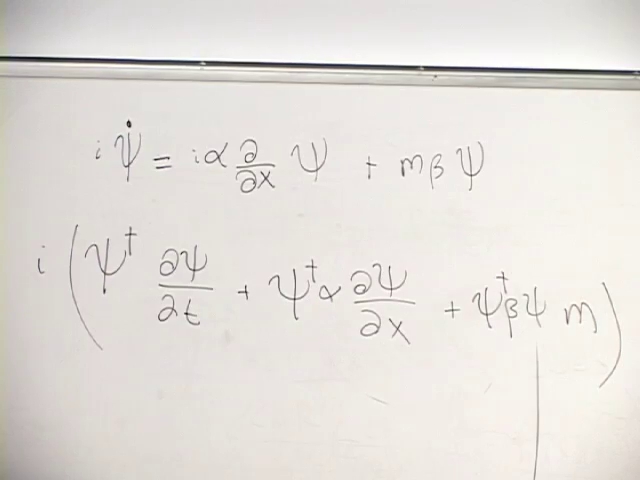
\includegraphics[width=0.76\textwidth]{lecture_09_figure_05.png}
\caption{Terme mit zeitlicher und räumlicher Ableitung sowie der Massenterm in der Diskussion des Dirac-Feldes.}
\lectureframe{00:25:37}
\end{figure}

\begin{classroomqa}
\lecturetimestamp{00:26:37}
\audiencequestion{Ist die Klammer in der versuchsweise angegebenen Dirac-Lagrangedichte richtig gesetzt, sodass \(i\) den gesamten Ausdruck multipliziert?}
\lecturerresponse{Die genaue Stellung wird hier nicht mit Sicherheit festgelegt und ist für den strukturellen Punkt auch nicht erforderlich: Es gibt eine Lagrangedichte, aus der die Dirac-Gleichung folgt.}
\end{classroomqa}

Fügen wir nun ein Skalarfeld \(\phi\) hinzu. Das naive Produkt \(\Psi^\dagger\Psi\,\phi\) ist kein Lorentz-Skalar. Setzt man stattdessen dieselbe Dirac-Matrix ein, die auch im Massenterm vorkommt, erhält man
\begin{equation}
\mathcal L_{\mathrm{int}}
\propto
\Psi^\dagger\beta\Psi\,\phi.
\end{equation}
Äquivalent dazu ist \(\Psi^\dagger\beta\Psi\) das skalare Dirac-Bilinear. Die Variation der vollständigen Lagrangedichte fügt der Dirac-Gleichung einen zu \(\phi\) proportionalen Term und der Skalarfeldgleichung eine zu \(\Psi^\dagger\beta\Psi\) proportionale Quelle hinzu. Die beiden Felder streuen einander.

\begin{classroomqa}
\lecturetimestamp{00:28:03}
\audiencequestion{Ist das in die Skalar--Fermion-Wechselwirkung eingesetzte \(\beta\) dasselbe \(\beta\), das auch im Dirac-Massenterm vorkommt?}
\lecturerresponse{Ja. Es ist dieselbe Dirac-Matrix.}
\end{classroomqa}

Der Vergleich
\begin{equation}
m\Psi^\dagger\beta\Psi
\qquad\hbox{and}\qquad
\Psi^\dagger\beta\Psi\,\phi
\end{equation}
lässt die Kopplung wie einen Massenparameter erscheinen, der durch ein Skalarfeld ersetzt wurde. Auf diese Beobachtung kommen wir gegen Ende zurück, wenn wir ein Feld mit einem von null verschiedenen Vakuumwert betrachten.

Bis hierher war die Deutung klassisch: Wellenpakete streuen andere Wellenpakete. Dieselbe Algebra erhält eine präzisere Teilchenbedeutung, wenn die Felder zu Operatoren werden.

\section{Was die Potenzen von Quantenfeldern bewirken}

Ein reelles Skalar-Quantenfeld enthält sowohl Erzeugungs- als auch Vernichtungsoperatoren. Schematisch gilt
\begin{equation}
\phi(x)\sim A^+(x)+A^-(x),
\end{equation}
wobei \(A^+\) ein Quant erzeugt und \(A^-\) eines vernichtet. Daher umfasst \(\phi^3(x)\) vier Arten lokaler Prozesse:
\begin{equation}
\phi^3
\sim
(A^+)^3+(A^+)^2A^-+A^+(A^-)^2+(A^-)^3,
\end{equation}
wobei in dieser schematischen Betrachtung die Details der Operatorreihenfolge und numerische Koeffizienten unterdrückt sind. Die vier Änderungen der Teilchenzahl lauten
\begin{equation}
3\longrightarrow0,
\qquad
0\longrightarrow3,
\qquad
2\longrightarrow1,
\qquad
1\longrightarrow2.
\end{equation}
Alle drei Feldfaktoren wirken am selben Punkt \(x\). Ein einzelner kubischer Term umfasst somit die Vernichtung dreier Teilchen, die Erzeugung dreier Teilchen, die Fusion zweier Quanten zu einem und die Aufspaltung eines Quants in zwei. In einer physikalischen Amplitude können einige dieser lokalen Deutungen später durch Energie--Impuls-Erhaltung ausgeschlossen werden; sie sind jedoch alle im Operatorprodukt selbst enthalten.

Die quadratischen freien Terme haben eine andere Funktion. Unterdrücken wir zunächst die Normierung des Unterschieds zwischen benachbarten Punkten \(x\) und \(x'\):
\begin{equation}
\partial_x\phi
\ \propto\
\phi(x)-\phi(x').
\end{equation}
Quadrieren und Ausmultiplizieren ergibt folgende Termstruktur:
\begin{align}
\frac12(\partial_x\phi)^2
&\ \propto\
\frac12\bigl[\phi(x)-\phi(x')\bigr]^2
\\
&=
\frac12\phi(x)^2
+\frac12\phi(x')^2
-\phi(x)\phi(x').
\end{align}
Jedes Quadrat an einem einzelnen Punkt lässt mehrere Operator-Deutungen zu: Es kann zwei Quanten erzeugen, zwei vernichten oder am selben Punkt eines vernichten und wieder erzeugen. Diese Terme transportieren kein Teilchen. Der gemischte Term kann ein Quant bei \(x'\) vernichten und eines bei \(x\) erzeugen oder umgekehrt. Er wirkt daher wie ein Hüpfterm zwischen nächsten Nachbarn. Wiederholte Faktoren transportieren ein Teilchen von \(x\) nach \(x'\), dann nach \(x''\) und so weiter. Quadratische Ableitungsterme bestimmen die freie Ausbreitung; kubische und höhere Terme streuen, erzeugen und vernichten Teilchen.

\begin{classroomqa}
\lecturetimestamp{00:36:07}
\audiencequestion{Muss die Differenzdarstellung der Ableitung den Abstand \(x-x'\) enthalten?}
\lecturerresponse{Ja. Bezeichnet man den Abstand mit \(L\), ergibt das Quadrieren der Differenz den Faktor \(L^{-2}\). Dieser Zahlenfaktor ändert den Koeffizienten, aber nichts an der Deutung als Hüpfterm.}
\end{classroomqa}

Mit wieder eingesetztem Abstand ergibt sich
\begin{align}
\frac12(\partial_x\phi)^2
&\longrightarrow
\frac{1}{2L^2}\bigl[\phi(x)-\phi(x')\bigr]^2
\\
&=
\frac{1}{2L^2}\phi(x)^2
+\frac{1}{2L^2}\phi(x')^2
-\frac{1}{L^2}\phi(x)\phi(x').
\end{align}

Auch der Massenterm ist quadratisch, enthält aber keine Ableitung:
\begin{equation}
\frac12m^2\phi(x)^2.
\end{equation}
In der Einteilchen-Deutung wird ein ankommendes Quant am selben Punkt absorbiert und wieder emittiert. Es bewegt das Quant nicht, sondern gewichtet – oder zählt in diesem Sinn – dessen Anwesenheit dort. Dasselbe Operatorquadrat enthält auch die Deutungen mit zwei Erzeugungen und mit zwei Vernichtungen. Für die Bewegung ist also entscheidend, ob ein gemischter Term benachbarte Punkte verbindet oder eine Masseneinfügung innerhalb eines Punktes wirkt.

\section{Der lokale Vertex der Quantenelektrodynamik}

Diese elementaren Skizzen von Teilchenprozessen bilden den Anfang der Feynman-Diagramme. Das zentrale Beispiel ist die Quantenelektrodynamik, die Theorie der Elektronen, Positronen und Photonen.

Die Dirac-Gleichung besitzt Moden mit positiver und negativer Energie. In der älteren Sprache enthält \(\Psi\) Vernichtungsoperatoren für beide Arten von Moden, während \(\Psi^\dagger\) die entsprechenden Erzeugungsoperatoren enthält. Die Entfernung eines Elektrons mit negativer Energie wird als Erzeugung eines Positrons mit positiver Energie umgedeutet. Nach dieser Umbenennung lautet die nützliche schematische Zerlegung
\begin{align}
\Psi
&\sim
C^-_{e^-}+C^+_{e^+},
\\
\Psi^\dagger
&\sim
C^+_{e^-}+C^-_{e^+}.
\end{align}
Somit vernichtet \(\Psi\) ein Elektron oder erzeugt ein Positron, während \(\Psi^\dagger\) ein Elektron erzeugt oder ein Positron vernichtet. Diese Kurzschreibweise enthält weder Normierung noch Spinindex oder Impulsintegral.

Die QED-Wechselwirkung koppelt den Dirac-Strom an das elektromagnetische Viererpotential. In der hier verwendeten Komponenten-Schreibweise hat sie folgende Struktur:
\begin{equation}
\mathcal L_{\mathrm{QED,int}}
\sim
e\left(
\Psi^\dagger\Psi\,A_0
+
\Psi^\dagger\boldsymbol{\alpha}\Psi\mathbin{\boldsymbol{\cdot}}\mathbf A
\right),
\end{equation}
wobei
\begin{equation}
J^0=\Psi^\dagger\Psi,
\qquad
\mathbf J=\Psi^\dagger\boldsymbol{\alpha}\Psi.
\end{equation}
Das Symbol \(\sim\) ist wichtig: Das relative Vorzeichen zwischen zeitlichem und räumlichem Term hängt von der Metrik- und Viererpotential-Konvention ab. Die invariante Aussage lautet, dass der Viererstrom mit dem Viererpotential kontrahiert wird.\editorialnote{Die Vorlage legt die zeitliche und räumliche Komponente des Stroms fest, bestimmt aber keine Metrik-Konvention für die Kontraktion der Komponenten.}

Das Photonenfeld \(A_\mu\) selbst enthält Erzeugungs- und Vernichtungsoperatoren für Photonen. Sein Vektorcharakter trägt außerdem die Polarisation des Photons--- – eine kleine Richtungs``markierung'' zusätzlich zu seinem Impuls.

\begin{classroomqa}
\lecturetimestamp{00:44:28}
\audiencequestion{Wie kann die Wechselwirkung ein Skalar sein, wenn \(A_\mu\) ein Vektor ist und der Fermionfaktor zunächst wie ein Skalar aussieht?}
\lecturerresponse{Auch die Fermionen liefern einen Vierervektor: \(\Psi^\dagger\Psi\) ist seine zeitliche Komponente und \(\Psi^\dagger\boldsymbol\alpha\Psi\) seine räumliche Komponente. Die Kontraktion dieses Stroms mit \(A_\mu\) ergibt einen Skalar.}
\end{classroomqa}

Multipliziert man die Operatorinhalte von \(\Psi^\dagger\), \(\Psi\) und \(A_\mu\), ergeben sich vier vertraute Deutungen eines lokalen Vertex:
\begin{enumerate}
\item Ein Elektron emittiert ein Photon;
\item ein Elektron absorbiert ein Photon;
\item ein Elektron und ein Positron annihilieren zu einem Photon;
\item ein Photon erzeugt ein Elektron--Positron-Paar.
\end{enumerate}
Bei der ersten Deutung vernichtet \(\Psi\) das einlaufende Elektron, \(\Psi^\dagger\) erzeugt das auslaufende Elektron und das Photonenfeld erzeugt das Photon. Wählt man den Vernichtungsanteil des Photons, erhält man die Absorption. Wählt man die Positron-Anteile, erhält man Paarvernichtung oder Paarerzeugung. Ein lokaler Term enthält die ganze Familie.

In einem Diagramm mit Fermionfluss zeigt der Pfeil auf einer Positronlinie entgegen der Ausbreitungsrichtung des Positrons. Bei dieser Konvention läuft der Fermionpfeil stetig durch jeden zulässigen QED-Vertex. Die vier Deutungen unterscheiden sich dadurch, dass äußere Linien zwischen der einlaufenden und der auslaufenden Seite verschoben werden, nicht dadurch, dass die Fermionflusslinie unterbrochen wird.

Jede dieser Deutungen trägt denselben Koeffizienten \(e\), die elektrische Ladung in der hier verwendeten mikroskopischen Konvention. Dieser Koeffizient ist die elektrische Ladung \(e\), nicht die Feinstrukturkonstante, obwohl beide eng zusammenhängen. Die Vertexamplitude ist proportional zu \(e\); berücksichtigt man alle kinematischen und Normierungsfaktoren, ist die entsprechende Wahrscheinlichkeit proportional zu \(e^2\).

\begin{classroomqa}
\lecturetimestamp{00:49:44}
\audiencequestion{Hat die Deutung Photon zu Elektron--Positron denselben Koeffizienten wie die anderen Deutungen des Vertex?}
\lecturerresponse{Ja. Sie enthält denselben Koeffizienten für die elektrische Ladung \(e\).}
\end{classroomqa}

\begin{classroomqa}
\lecturetimestamp{00:49:59}
\audiencequestion{Muss es einen Skalierungsfaktor geben, da eine Wahrscheinlichkeit keine Einheit hat?}
\lecturerresponse{In der hier verwendeten natürlichen mikroskopischen Konvention ist die Ladung \(e\) dimensionslos. Sie bestimmt die Größenordnung der Amplitude, ihr Quadrat die Größenordnung der Wahrscheinlichkeit.}
\end{classroomqa}

Ein konkretes Bild: Ein Elektron trifft auf eine Wand und kommt abrupt zum Stillstand. Mit einer gewissen Wahrscheinlichkeit werden Energie und Impuls in Form eines Photons abgegeben. Der elementare elektromagnetische Faktor in der Strahlungsamplitude ist \(e\); daher enthält die entsprechende Wahrscheinlichkeit \(e^2\). Diese Aussage isoliert den Kopplungsfaktor; die tatsächliche Wahrscheinlichkeit hängt auch vom Zustand des Elektrons und von der Kinematik ab.

\begin{figure}[htbp]
\centering
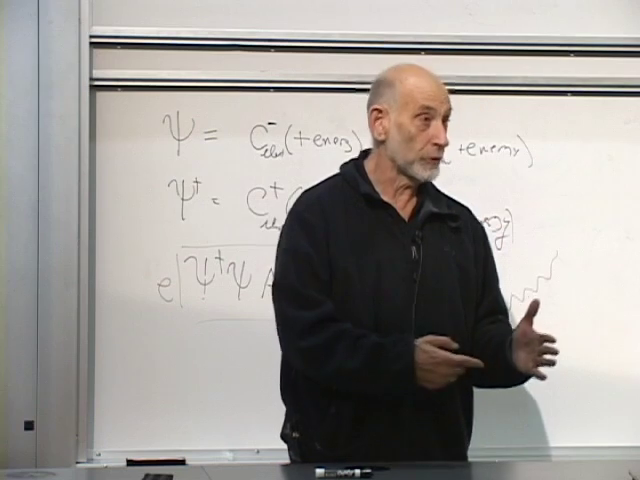
\includegraphics[width=0.78\textwidth]{lecture_09_figure_06.png}
\caption{Operatorinhalt von \(\Psi\) und \(\Psi^\dagger\) für Elektronen und Positronen sowie eine Skizze der Elektron--Photon-Wechselwirkung.}
\lectureframe{00:50:39}
\end{figure}

\begin{classroomqa}
\lecturetimestamp{00:51:15}
\audiencequestion{Hat die elektrische Ladung eine Einheit?}
\lecturerresponse{In der hier verwendeten natürlichen mikroskopischen Konvention nicht. Makroskopische Ladung wird oft in Coulomb angegeben, aber in der Teilchentheorie misst man die Ladung relativ zu einer gewählten elementaren Einheit. In Planck-Einheiten oder anderen natürlichen Einheiten werden die Größen als reine Zahlen ausgedrückt.}
\end{classroomqa}

Der Unterschied beruht auf Konventionen und Maßstäben. Coulomb eignet sich zur Angabe des Stroms in Leitungen; eine dimensionslose Kopplung ist für mikroskopische Amplituden praktisch.\editorialnote{Eine kurze Frage bei 00:52:37--00:53:15 zur ``Gruppierung'' ladungstragender Terme ist stark beschädigt und führte zu keiner eindeutigen Konstruktion.}

Alle drei Felder der elementaren QED-Wechselwirkung werden am selben Raumzeitpunkt ausgewertet. Dem Vertex selbst ist keine interne Zeitverzögerung zugeordnet.

\begin{classroomqa}
\lecturetimestamp{00:53:19}
\audiencequestion{Finden die Absorption und Wiederaussendung des Elektrons sowie die Emission des Photons gleichzeitig statt, oder enthält die Gleichung eine Verzögerung?}
\lecturerresponse{Am elementaren Vertex werden alle Operatoren am selben Raumzeitpunkt ausgewertet. Der grundlegende Prozess enthält daher keine Verzögerung zwischen diesen Vorgängen.}
\end{classroomqa}

\begin{classroomqa}
\lecturetimestamp{00:53:57}
\audiencequestion{Muss jede Erhaltungsgröße einzeln erhalten bleiben?}
\lecturerresponse{Ja. Die elektrische Ladung ist eine der Größen, die einzeln erhalten bleiben müssen.}
\end{classroomqa}

Die Ladungserhaltung ist sowohl im Diagramm als auch in der Algebra zu erkennen. Ein Prozess, der ein einlaufendes Elektron in ein auslaufendes Positron umwandelt, würde die Ladung umkehren und ist kein zulässiger QED-Vertex. Ist die Zeit nach oben aufgetragen, weist der Elektronenpfeil nach oben und der Positronenpfeil nach unten; am zulässigen Vertex verläuft immer ein Fermionpfeil durchgehend. Algebraisch enthält die Wechselwirkung ein \(\Psi\) und ein \(\Psi^\dagger\). Der erste erhöht die Ladung um eine Einheit, wenn er ein Elektron vernichtet oder ein Positron erzeugt; der zweite senkt sie um eine Einheit. Die Wirkungen heben sich auf.

\begin{classroomqa}
\lecturetimestamp{00:56:05}
\audiencequestion{Ist der eingerahmte Ausdruck für Elektron--Photon die gesamte QED-Lagrangedichte?}
\lecturerresponse{Nein. Es ist der Wechselwirkungsterm. Die quadratischen freien Photonenterme und die quadratischen Dirac-Terme, die die Ausbreitung bestimmen, sind nicht angegeben.}
\end{classroomqa}

\begin{classroomqa}
\lecturetimestamp{00:56:35}
\audiencequestion{Wird eine klassische Lagrangedichte hergeleitet, während man eine Quantен-Lagrangedichte errät und überprüft, und bleibt die Struktur kinetische Energie minus potenzielle Energie in der Quantenmechanik erhalten?}
\lecturerresponse{Das Muster kinetische Energie minus potenzielle Energie bleibt erhalten: Zeitliche Ableitungen liefern die kinetische Form, räumliche Gradienten verallgemeinern sie, und undifferenzierte Feldterme liefern die potenzielle Form. Die Quanten-Lagrangedichte ist die grundlegendere Beschreibung. In einem Zustand mit sehr vielen Quanten erzeugt dieselbe Lagrangedichte die klassischen Wellengleichungen. Kandidaten für Lagrangedichten werden anhand physikalischer Prinzipien und tiefer gehender Theorien vorgeschlagen und anschließend durch Stoßexperimente bestätigt oder verworfen.}
\end{classroomqa}

Der Grenzfall großer Besetzungszahlen erklärt, warum derselbe Ausdruck sowohl eine Quantenteilchentheorie als auch ihre klassischen Wellen beschreiben kann. Diese Übereinstimmung ist kein nachträglich hinzugefügtes separates Wunder; das klassische Feld ist das kollektive Verhalten vieler Quanten. Umgekehrt legen experimentelle Stöße die elementaren Vertizes so direkt offen, dass sich die Wechselwirkungen der QED und des Standardmodells mit großer Präzision bestimmen lassen.

\section{Kreuzung und Erhaltungssätze in der Raumzeit}

Die Linien eines lokalen Vertex können zwischen einlaufenden und auslaufenden Positionen gekreuzt werden. Eine auslaufende Teilchenlinie, die auf die einlaufende Seite verschoben wird, wird als ihr Antiteilchen umgedeutet und umgekehrt. In diesem Sinn erlaubt derselbe Elektron--Positron--Photon-Operator Deutungen für Emission, Absorption, Paarvernichtung, Paarerzeugung und sogar einen lokalen Prozess, bei dem alle Teilchen einlaufen.

\begin{classroomqa}
\lecturetimestamp{00:59:34}
\audiencequestion{Bleibt ein Diagramm eines elementaren Vertex nach einer Drehung ein zulässiges lokales Prozessbild?}
\lecturerresponse{Ja. Seine äußeren Linien können zwischen den einlaufenden und auslaufenden Positionen verschoben werden, wobei das Teilchen--Antiteilchen entsprechend umgedeutet wird.}
\end{classroomqa}

Die lokale Deutung des Operators ist noch kein vollständiger physikalischer Prozess. Seine Amplitude muss über alle Raumzeitpunkte integriert werden, an denen der Vertex auftreten könnte. Das Zeitintegral erzwingt die Energieerhaltung, das Raumintegral die Impulserhaltung. Ein Bild, in dem ein Elektron, ein Positron und ein Photon gemeinsam im Vakuum verschwinden, ist als formale lokale Deutung enthalten; die integrierte Amplitude verschwindet jedoch, weil der Prozess Energie und Impuls nicht erhalten kann.

\begin{classroomqa}
\lecturetimestamp{01:00:30}
\audiencequestion{Bedeutet das Bild mit allen einlaufenden Teilchen, dass ein Elektron, ein Positron und ein Photon spurlos verschwinden können?}
\lecturerresponse{Es ist eine Deutung des lokalen Operators, aber die physikalische Amplitude umfasst eine Integration über die Position des Vertex. Diese Integrale erzwingen die Erhaltung von Energie und Impuls, sodass die kinematisch verbotene Amplitude null ist.}
\end{classroomqa}

\begin{classroomqa}
\lecturetimestamp{01:01:57}
\audiencequestion{Gibt es auch die umgekehrte Deutung, bei der aus dem Vakuum ein Elektron--Positron--Photon entsteht, und verschwinden ausgeschlossene Prozesse nach der Integration?}
\lecturerresponse{Auch diese umgekehrte lokale Deutung ist enthalten. Die Integration über Raum und Zeit unterdrückt jeden Prozess, der mit den Erhaltungssätzen unvereinbar ist.}
\end{classroomqa}

Die Ableitungen in der Lagrangedichte passen zur Operatorentwicklung, ohne die Erzeugungs- und Vernichtungssymbole selbst abzuleiten. Ein Feld hat schematisch die Form
\begin{equation}
\Psi(x)
\sim
\int d^3k\,
\bigl[
C(\mathbf k)e^{i\mathbf k\cdot\mathbf x-i\omega t}
+\cdots
\bigr].
\end{equation}
Die Operatoren \(C(\mathbf k)\) sind Koeffizienten in dieser Raumzeitentwicklung. Die Ableitungen wirken auf die ebenen Wellen und liefern \(\mathbf k\) oder \(\omega\).

\begin{classroomqa}
\lecturetimestamp{01:02:27}
\audiencequestion{Wird beim Ableiten einer Feldentwicklung der Erzeugungsoperator selbst abgeleitet?}
\lecturerresponse{Nein. Die Erzeugungs- und Vernichtungsoperatoren hängen in dieser Entwicklung nicht von der Raumzeitkoordinate ab. Die Ableitungen wirken auf die Exponentialfaktoren und liefern Impuls und Frequenz.}
\end{classroomqa}

\section{Nukleonen und Pionen als effektive Theorie}

Dieselbe Sprache lässt sich auf Protonen, Neutronen und Pionen anwenden. Protonen und Neutronen sind Fermionen, die durch die Felder \(\Psi_p\) und \(\Psi_n\) dargestellt werden. Für diese Diskussion der Wechselwirkungen behandeln wir die Pionenfelder als Skalarfelder in drei Ladungszuständen:
\begin{equation}
\pi^+,
\qquad
\pi^-,
\qquad
\pi^0.
\end{equation}
Das Proton und \(\pi^+\) tragen jeweils eine positive Einheit elektrischer Ladung, das \(\pi^-\) eine negative Einheit; Neutron und \(\pi^0\) sind ungeladen. Auf einer tieferen Ebene sind Pionen Quark--Antiquark-Systeme; zunächst kann man diese innere Struktur jedoch außer Acht lassen.

Eine schematische, ladungserhaltende Liste von Produkten aus Nukleon--Pion-Feldern lautet
\begin{equation}
\mathcal L_{N\pi}
\sim
\left\{
\Psi_p^\dagger\Psi_n\,\pi^+,\;
\Psi_n^\dagger\Psi_p\,\pi^-,\;
\Psi_p^\dagger\Psi_p\,\pi^0,\;
\Psi_n^\dagger\Psi_n\,\pi^0
\right\}.
\end{equation}
Dargestellt werden nur der Feldinhalt und die Ladungszuordnungen; relative Koeffizienten, Vorzeichen und die Spinormatrixstruktur sind hier nicht festgelegt. Die Ladung des ersten Pionfeldes lässt sich durch eine konkrete Deutung bestimmen: Ein Neutron kann zusammen mit einem positiven Pion ein Proton ergeben; ein negatives Pion an dieser Stelle würde dagegen negative einlaufende Ladung in positive auslaufende Ladung umwandeln. Der konjugierte Term ergibt den entgegengesetzten geladenen Prozess.\editorialnote{Das Vorzeichen des Pions wird in der Vorlage mehrfach korrigiert, bevor das hier gezeigte ladungserhaltende Paar erreicht ist; die angegebene Reihenfolge gibt diese abschließende schematische Struktur wieder.}

Jeder Term lässt wiederum mehrere gekreuzte Deutungen zu. Verschiebt man ein auslaufendes Neutron auf die einlaufende Seite, wird es zu einem einlaufenden Antineutron. Der geladene Vertex kann daher die Verbindung eines Protons und eines Antineutrons zu einem \(\pi^+\) beschreiben, ebenso wie Prozesse der Form \(p\to n+\pi^+\), sofern die Kinematik sie zulässt. Die neutralen Terme erlauben einem Proton oder Neutron, ein \(\pi^0\) zu emittieren oder zu absorbieren. Die Ladungserhaltung wählt die zulässige Familie aus; Energie, Impuls und weitere Symmetrien bestimmen, welcher Prozess darin bei einem bestimmten Experiment auftreten kann.

Diese effektive Beschreibung war nützlich, bevor man die Quark-Unterstruktur kannte. Sie bleibt immer dann nützlich, wenn eine Sonde diese Struktur nicht auflösen kann. Ein Proton besitzt eine räumlich ausgedehnte Verteilung seiner Bestandteile, ähnlich wie ein Atom eine innere Struktur hat, allerdings auf viel kleinerer Skala. Überträgt ein Experiment zu wenig Impuls, um das Proton aufzubrechen oder seine Struktur aufzulösen, kann man es als punktförmiges Teilchen mit eigenem Feld behandeln. Bei einem Stoß mit ausreichend hoher Energie werden die Quarks sichtbar; dann reicht das punktförmige Protonenfeld nicht mehr aus.

Da das Proton geladen ist, besitzt es auch eine lokale Proton--Photon-Wechselwirkung, schematisch \(J_p^\mu A_\mu\), wobei \(J_p^\mu\) der Protonenstrom ist. Das Elektron hat eine entsprechende Elektron--Photon-Wechselwirkung. Ein Proton kann sich durch Emission eines Photons nicht in ein Neutron umwandeln: \(p\to n+\gamma\) verletzt die Ladungserhaltung.

\begin{classroomqa}
\lecturetimestamp{01:10:28}
\audiencequestion{Was geschieht, wenn ein Proton und ein Elektron wechselwirken?}
\lecturerresponse{Jedes geladene Teilchen besitzt einen Photonvertex. Das Proton kann ein Photon emittieren und dabei ein Proton bleiben; das Elektron kann das Photon absorbieren und dabei ein Elektron bleiben. Eine Proton--Elektron-Streuung setzt sich aus diesen beiden lokalen Vertizes und der Ausbreitung des Photons zwischen ihnen zusammen.}
\end{classroomqa}

\section{Lokalität und wiederholte elementare Prozesse}

Für den vollständigen Proton--Elektron-Austausch gibt es keinen speziellen nichtlokalen Term. Ein lokaler Vertex emittiert das Photon am Proton, quadratische Photonenterme transportieren es von einem benachbarten Punkt zum nächsten, und ein weiterer lokaler Vertex absorbiert es am Elektron. Der ausgedehnte Prozess ist ein Produkt dieser elementaren Bestandteile.
\begin{equation}
\begin{aligned}
\bigl[J_p^\mu A_\mu\bigr](x_p)
&\longrightarrow
\underbrace{x_p\to x_1\to x_2\to\cdots\to x_e}_{\text{quadratic photon propagation}}
\\
&\longrightarrow
\bigl[J_e^\nu A_\nu\bigr](x_e).
\end{aligned}
\end{equation}
Die Pfeile in dieser schematischen Kette stehen für aufeinanderfolgende Einfügungen an benachbarten Punkten, nicht für eine neue nichtlokale Wechselwirkung.

\begin{classroomqa}
\lecturetimestamp{01:12:06}
\audiencequestion{Wie würde man die Lagrangedichte für den gesamten Proton--Elektron-Austausch schreiben?}
\lecturerresponse{Für den gesamten ausgedehnten Vorgang fügt man keinen eigenen Term hinzu. Er setzt sich aus einem lokalen Proton--Photon-Scheitel, wiederholten quadratischen Ausbreitungstermen und einem lokalen Elektron--Photon-Scheitel zusammen.}
\end{classroomqa}

Die lokale Struktur hat zwei Formen. Ein undifferenzierter Wechselwirkungsterm wirkt an einem einzelnen Raumzeitpunkt. Ein Ableitungsterm, ausgedrückt als endliche Differenz, verbindet diesen Punkt nur mit einem benachbarten Punkt. Keine der beiden Formen überträgt ein Teilchen direkt über eine endliche Entfernung. Die Ausbreitung über große Entfernungen setzt sich aus vielen infinitesimalen Schritten zusammen; eine elementare Fernwirkung gibt es nicht.

\begin{classroomqa}
\lecturetimestamp{01:14:36}
\audiencequestion{Enthält die Lagrangedichte nur Terme an jeweils einem Punkt?}
\lecturerresponse{Wechselwirkungsterme wirken an einem Punkt. Ableitungsterme verbinden einen Punkt mit einem infinitesimal benachbarten Punkt. Emission, viele Schritte zwischen benachbarten Punkten und Absorption ergeben zusammen einen Austausch über eine endliche Entfernung.}
\end{classroomqa}

\begin{classroomqa}
\lecturetimestamp{01:15:36}
\audiencequestion{Sind alle Bestandteile des ausgedehnten Vorgangs enthalten, und bedeutet ihre Verkettung Multiplikation?}
\lecturerresponse{Ja. Jeder elementare Emissions-, Schritt- oder Absorptionsvorgang ist in der Lagrangedichte kodiert. Produkte wiederholter Einsetzungen verknüpfen diese Bestandteile zu dem umfassenderen Vorgang.}
\end{classroomqa}

Die hier betrachtete relativistische Quantenfeldtheorie setzt die Raumzeit voraus, auf der ihre Felder definiert sind. Sie ist nicht mit einer vollständigen Quantentheorie einer dynamischen Raumzeitgeometrie zu verwechseln.

\begin{classroomqa}
\lecturetimestamp{01:16:28}
\audiencequestion{Gilt diese Verkettung auch in einem stark relativistischen Umfeld, etwa in der Nähe des Horizonts eines Schwarzen Lochs?}
\lecturerresponse{Die Erweiterung auf Schwarze Löcher liegt außerhalb des Geltungsbereichs dieser Konstruktion. Die hier verwendete Quantenfeldtheorie liefert für sich genommen keine vollständige Beschreibung der Dynamik Schwarzer Löcher, bei der die Gravitation wesentlich ist.}
\end{classroomqa}

Ein Feld ist ein Operator für einen elementaren lokalen Vorgang. Ein Feldfaktor kann ein Teilchen absorbieren oder eines emittieren. Ein Produkt aus zwei Faktoren kann am selben Punkt ein Teilchen absorbieren und ein anderes emittieren; höhere Produkte können den Teilcheninhalt weiter verändern. Produkte lokaler Operatoren fügen diese Vorgänge zu Abläufen zusammen. In der Raumzeit wird Bewegung durch Absorption in einem kleinen Gebiet, erneute Emission in ein benachbartes Gebiet, eine weitere Absorption und eine weitere Emission dargestellt. Lässt man die Schrittweite gegen null gehen und zugleich die Schrittzahl wachsen, erhält man die kontinuierliche Bahn.

\begin{classroomqa}
\lecturetimestamp{01:17:30}
\audiencequestion{Wie sind Felder, Abstände und Zeit in diesem Bild lokaler Schritte zu verstehen?}
\lecturerresponse{Felder sind Operatoren für lokale Absorption und Emission. Produkte fügen diese elementaren Vorgänge zusammen, und die Bewegung durch die Raumzeit entsteht aus infinitesimalen Schritten zwischen benachbarten Punkten, bevor man den Kontinuumsgrenzwert bildet.}
\end{classroomqa}

Ein regulierter Ausgangspunkt ist daher die Zerlegung der Raumzeit in kleine Zellen, denen die Feldoperatoren zugeordnet sind.\editorialnote{Die Formulierung der Frage aus dem Publikum bei 01:17:30--01:20:40 ist teilweise unverständlich; die sinngemäße Wiedergabe enthält nur das noch erkennbare Thema, während die Antwort zu lokalen Operatoren und aufeinanderfolgenden Raumzeitschritten klar ist.} Ableitungen werden zu Differenzen. Quadratische Kreuzterme verbinden benachbarte Zellen, während Massen- und Wechselwirkungsterme innerhalb einer Zelle wirken. Die Zellen dienen dazu, die Grenztheorie zu definieren; sie sind weder zusätzliche Teilchen noch eine neue physikalische Massenskala.

Spezialrelativistische Effekte müssen nicht bei jedem Schritt gesondert hinzugefügt werden. Ist die Lagrangedichte ein Lorentzskalar, so sind die daraus zusammengesetzten Amplituden Lorentz-invariant, und Effekte wie die Zeitdilatation folgen aus dieser Struktur.

\begin{classroomqa}
\lecturetimestamp{01:21:10}
\audiencequestion{Verursachen Bewegungen bei hohen Energien und die Zeitdilatation zusätzliche Probleme bei einem mehrstufigen Vorgang?}
\lecturerresponse{Eine gesonderte Korrektur ist nicht erforderlich. Ist die Lagrangedichte ein Lorentzskalar, sind relativistische Effekte wie die Zeitdilatation bereits im Ergebnis enthalten. Was genau mit der Frage gemeint ist, bleibt ansonsten unklar.}
\end{classroomqa}

Erzeugungs- und Vernichtungsoperatoren lassen sich in einer Ortsbasis oder in einer Impulsbasis darstellen. Ein Erzeugungsoperator im Ortsraum ist eine Fourier-Überlagerung von Erzeugungsoperatoren im Impulsraum und umgekehrt. Es gibt keinen Operator, der einen Zustand mit zugleich exakt festgelegtem Ort und exakt festgelegtem Impuls erzeugt. Eine scharfe Lokalisierung des Teilchens im Ort erfordert ein breites Impulsband; eine scharfe Lokalisierung im Impuls verteilt es über den Ort. Die Fourier-Beziehung zwischen den beiden Basen drückt in dieser Sprache die Unschärferelation aus.

\begin{classroomqa}
\lecturetimestamp{01:22:48}
\audiencequestion{Wie hängen Erzeugungs- und Vernichtungsoperatoren mit Ort, Impuls und der Unschärferelation zusammen?}
\lecturerresponse{Sie lassen sich als Funktionen des Ortes oder als Funktionen des Impulses darstellen. Die beiden Darstellungen sind Fourier-Transformationen voneinander. Ein scharf lokalisierter Zustand im Ort erfordert viele Impulse, während ein scharf lokalisierter Impulszustand über den Ort verteilt ist; es gibt keinen Erzeugungsoperator für zugleich scharfe Werte von \(x\) und \(p\).}
\end{classroomqa}

Die Zellkonstruktion lässt sich nun vollständig angeben. Man nummeriert die Zellen mit \(n\), ersetzt eine Ableitung durch eine endliche Differenz, etwa
\begin{equation}
\partial_\mu\phi(x)
\longrightarrow
\frac{\phi_{n+\hat\mu}-\phi_n}{a},
\end{equation}
und ordnet jede Feldart jeder Zelle zu. Ein quadratischer Kreuzterm entfernt ein Quant aus einer Zelle und erzeugt eines in einer Nachbarzelle. Die Kontinuumstheorie erhält man, indem man den Abstand \(a\) gegen null gehen lässt, nachdem die regulierten Ausdrücke definiert worden sind.
\begin{equation}
\underbrace{\phi_n\phi_{n+\hat\mu}}_{\text{hop }n\leftrightarrow n+\hat\mu},
\qquad
\underbrace{m^2\phi_n^2}_{\text{same-cell mass insertion}}.
\end{equation}

\begin{classroomqa}
\lecturetimestamp{01:25:16}
\audiencequestion{Lässt sich die Zerlegung der Raumzeit in Zellen vollständig durchführen?}
\lecturerresponse{Ja. Die Felder werden durch Zellen indiziert, Ableitungen werden zu endlichen Differenzen, und quadratische Terme lassen Teilchen zwischen benachbarten Zellen wechseln. Das Kontinuum erhält man, wenn die Zellgröße gegen null geht.}
\end{classroomqa}

Elektronen wechseln über ihre quadratischen Terme zwischen den Zellen, und Photonen tun dasselbe. Treffen ein Elektron und ein Photon in einer Zelle zusammen, kann die QED-Wechselwirkung das Elektron absorbieren und erneut emittieren und dabei das Photon erzeugen oder vernichten. Der skalare Massenterm lässt sich für dieselbe Zelle deuten: Ein Teilchen tritt in die Zelle ein und verlässt sie wieder, mit einem Koeffizienten proportional zu \(m^2\). Er bewirkt keinen Wechsel zwischen Zellen.

\begin{classroomqa}
\lecturetimestamp{01:28:18}
\audiencequestion{Hängt die Zellgröße mit dem Massenkoeffizienten zusammen?}
\lecturerresponse{Nein. Die Zellgröße ist ein Regulatorabstand, der letztlich gegen null geht; der Massenkoeffizient ist ein unabhängiger Parameter der Lagrangedichte.}
\end{classroomqa}

\begin{classroomqa}
\lecturetimestamp{01:28:43}
\audiencequestion{Ist das Multiplizieren der lokalen Faktoren eine gemeinsame Amplitudenkonstruktion über die Raumzeit hinweg und nicht bloß eine zeitliche Abfolge?}
\lecturerresponse{Ja. Die Zellen überdecken die Raumzeit, und ihre lokalen Beiträge verbinden sich über dieses Raumzeitgitter hinweg. Das Produkt liefert eine gemeinsame Amplitude für die erforderlichen lokalen Vorgänge und Ausbreitungsschritte.}
\end{classroomqa}

\section{Quellen, Detektoren und die Dynamik dazwischen}

Ein vollständiger Vorgang ist ein Ablauf in der Raumzeit. Seine Anfangsbedingung wird dadurch festgelegt, was der Experimentator vorbereitet, seine Endbedingung dadurch, was die Detektoren registrieren. Eine einfache Quelle ist ein heißer Glühfaden, der ein Elektron emittiert. Ein Feldoperator am Glühfaden erzeugt dieses einlaufende Elektron; Feldoperatoren an den Detektorpositionen beschreiben seine spätere Absorption.

\begin{classroomqa}
\lecturetimestamp{01:29:30}
\audiencequestion{Was ist die Anfangsphase eines solchen Raumzeitvorgangs?}
\lecturerresponse{Sie wird an den Quellen vorbereitet. Ein von einem heißen Glühfaden emittiertes Elektron ist ein einfaches Beispiel: Ein Feldoperator am Glühfaden erzeugt das Elektron, während Feldoperatoren an den Detektoren die abschließenden Absorptionsvorgänge festlegen.}
\end{classroomqa}

Dieselbe Konstruktion lässt sich ausgehend vom Vakuum formulieren. Erzeugungsoperatoren an den Quellen bauen den einlaufenden Zustand auf dem Vakuum auf. Den Detektoren zugeordnete Vernichtungsoperatoren wählen den auslaufenden Zustand aus. Diese Operatoren legen Randbedingungen fest; sie ersetzen nicht die Dynamik im gesamten Gebiet zwischen Quelle und Detektor.

\begin{classroomqa}
\lecturetimestamp{01:31:11}
\audiencequestion{Wäre es falsch, die Dynamik nur an den Emissionsorten und nicht im gesamten System anzusetzen?}
\lecturerresponse{Ja. Man geht vom Vakuum aus, verwendet Quellenoperatoren, um die einlaufenden Teilchen vorzubereiten, und Detektoroperatoren, um die Endteilchen auszuwählen. Dazwischen wirken wiederholte Einsetzungen der Lagrangedichte in der gesamten Raumzeit: Sie bewegen, erzeugen und vernichten Teilchen.}
\end{classroomqa}

Bei genügend vielen Einsetzungen können sich mehrere Teilchen gleichzeitig durch viele benachbarte Zellen bewegen; unterwegs können Teilchen auch erzeugt oder vernichtet werden. Die Anfangsoperatoren geben an, was eintritt, die Endoperatoren, was registriert wird, und die wiederholten Wirkungen der Lagrangedichte liefern alles dazwischen.

\begin{classroomqa}
\lecturetimestamp{01:33:24}
\audiencequestion{Werden die Orte der Einsetzungen integriert, wenn beliebig viele Lagrangedichte-Einsetzungen auftreten können?}
\lecturerresponse{Ja. Über ihre Raumzeitpositionen wird integriert. Die exakten Feynman-Regeln werden hier nicht hergeleitet; zunächst geht es darum, dass einfache lokale Feldausdrücke die elementaren Wechselwirkungen kodieren, aus denen ein vollständiger Vorgang zusammengesetzt wird.}
\end{classroomqa}

\section{Phasensymmetrie, Ladung und Amplituden}

Wenn man die elementaren Vorgänge in einer Lagrangedichte formuliert, werden auch ihre Symmetrien sichtbar. Betrachten wir eine globale Phasentransformation des Elektronenfeldes,
\begin{equation}
\Psi\longrightarrow e^{i\theta}\Psi,
\qquad
\Psi^\dagger\longrightarrow e^{-i\theta}\Psi^\dagger,
\qquad
A_\mu\longrightarrow A_\mu.
\end{equation}
Ein Term mit gleich vielen \(\Psi\) und \(\Psi^\dagger\) bleibt unverändert, weil sich die Phasen aufheben. Ein Term mit ungleicher Anzahl würde einen Phasenfaktor erhalten. Die Gleichheit dieser Anzahlen ist die algebraische Form der Ladungserhaltung.

Das ist ein zentraler Vorteil der Lagrangebeschreibung. Ihre Feldfaktoren zeigen die elementaren Vorgänge, ihre Kombinationen zeigen die Symmetrien, und die Symmetrien machen die Erhaltungssätze sichtbar. Wiederholte Einsetzungen entwickeln den vorbereiteten Anfangszustand zum ausgewählten Endzustand weiter. Das Ergebnis ist eine quantenmechanische Amplitude. Für eine exakte Berechnung braucht man die Feynman-Regeln, doch der strukturelle Gehalt ist bereits erkennbar: Lokale Operationen wiederholen sich in jeder durch die Erhaltungssätze erlaubten Ordnung.

\section{Feldmessungen und Kommutatoren}

Feldoperatoren haben weiterhin ihre übliche quantenmechanische Bedeutung als Operatoren. Ihre Eigenwerte sind mögliche Ergebnisse von Feldmessungen, und ihre Eigenvektoren beschreiben Zustände, die diesen Werten zugeordnet sind. Ein elektrisches Feld lässt sich untersuchen, indem man ein geladenes Teilchen hineinbringt und beobachtet, wie es beschleunigt wird.

\begin{classroomqa}
\lecturetimestamp{01:37:06}
\audiencequestion{Haben Eigenwerte und Eigenvektoren von Feldoperatoren ihre übliche quantenmechanische Bedeutung?}
\lecturerresponse{Ja. Eigenwerte sind mögliche Messwerte des Feldes, und Felder lassen sich anhand ihrer Wirkung auf Teilchen untersuchen. Kommutatoren bestimmen, welche Einschränkungen für gleichzeitige Messungen gelten.}
\end{classroomqa}

Die triviale Identität
\begin{equation}
[\phi(x),\phi(x)]=0
\end{equation}
löst die Messfrage nicht. Man muss zwei Observablen und ihre raumzeitliche Beziehung angeben. Ein Feld und sein konjugierter Impuls bilden ein kanonisches, nicht kommutierendes Paar, und Feldoperatoren an zeitartig getrennten Punkten müssen nicht kommutieren; lokale bosonische Felder an raumartig getrennten Punkten kommutieren dagegen, wie es die Lokalität verlangt. Der bekannte Zusammenhang zwischen Kommutatoren und Unschärfe gilt also auch hier, aber erst, nachdem das Operatorpaar korrekt bestimmt worden ist.\editorialnote{Die Quelle stellt die Nichtkommutativität an verschiedenen Punkten zu allgemein dar. Diese Einschränkung bewahrt den Bezug zur Messfrage und berücksichtigt zugleich die Mikrokausalität raumartig getrennter lokaler bosonischer Felder.}

\begin{classroomqa}
\lecturetimestamp{01:39:57}
\audiencequestion{Misst man das elektrische oder elektromagnetische Feld in Volt oder in Volt pro Meter?}
\lecturerresponse{Das elektrische Feld misst man in Volt pro Meter. Volt und Meter sind nicht die hilfreichste Sprache für mikroskopische Feldvorgänge, die sich natürlicher anhand von Photonen beschreiben lassen. Umgekehrt ist die Quantenfeldtheorie nicht das geeignete Mittel, um zu entscheiden, wie man ein Haus bewässert.}
\end{classroomqa}

Die in einer Beschreibung natürlichen Einheiten müssen in einer anderen nicht besonders anschaulich sein. Volt und Volt pro Meter eignen sich für makroskopische Apparaturen; für mikroskopische Vorgänge passen Erzeugung und Vernichtung von Photonen.

\begin{classroomqa}
\lecturetimestamp{01:41:10}
\audiencequestion{Ist die zentrale Idee, dass Terme der Lagrangedichte Bausteine sind, die sich zu größeren Vorgängen verbinden?}
\lecturerresponse{Ja. Elementare Vorgänge wiederholen sich von einem Punkt zum nächsten. Jedes Grundelement wirkt an einem einzelnen Raumzeitpunkt oder verbindet benachbarte Punkte durch einen Ableitungsterm. Eine scheinbar nichtlokale Ausbreitung entsteht aus diesen lokalen Schritten; eine elementare Fernwirkung gibt es nicht.}
\end{classroomqa}

\section{Produkte lokaler Vorgänge und Summen über Wege}

Es gibt eine kompakte heuristische Darstellung für die Wiederholung lokaler Vorgänge. Man zerlegt die Raumzeit in Zellen und schreibt
\begin{equation}
\prod_x\bigl(1+\mathcal L_I(x)\bigr),
\end{equation}
wobei \(x\) die Zellen bezeichnet und \(\mathcal L_I(x)\) die lokale Wechselwirkungslagrangedichte ist. Dies ist nicht die exakte Kontinuumsformel. Es handelt sich um einen kombinatorischen Ersatz, der sichtbar macht, wie Produkte jede erlaubte Auswahl lokaler Vorgänge erzeugen.

\begin{classroomqa}
\lecturetimestamp{01:42:18}
\audiencequestion{Lassen sich viele Schritte der Erzeugung, Ausbreitung und Vernichtung in einem Ausdruck zusammenfassen?}
\lecturerresponse{Heuristisch multipliziert man für jede Raumzeitzelle einen Faktor \(1+\mathcal L_I(x)\). Beim Ausmultiplizieren des Produkts entstehen Terme für keinen Vorgang, für einen Vorgang an einem beliebig ausgewählten Punkt oder für Vorgänge an mehreren Punkten.}
\end{classroomqa}

Für zwei Zellen gilt
\begin{align}
\bigl(1+\mathcal L_I(x)\bigr)
\bigl(1+\mathcal L_I(x')\bigr)
&=
1+\mathcal L_I(x)+\mathcal L_I(x')
\notag\\
&\quad{}+\mathcal L_I(x)\mathcal L_I(x').
\end{align}
Der erste Term bedeutet, dass keine der beiden Wechselwirkungen stattfindet. Die nächsten beiden Terme setzen je eine elementare Wechselwirkung an \(x\) beziehungsweise an \(x'\) an. Der letzte Term enthält Wechselwirkungen an beiden Punkten. Bei vielen Faktoren gibt es Terme mit einem, zwei, drei und mehr Punkten. Ein Term mit mehreren Scheiteln kann beispielsweise zwei einlaufende Teilchen beschreiben, die drei auslaufende Teilchen erzeugen.

Auch quadratische Ausbreitungsterme gehen in dieselbe Konstruktion ein. Eine Verschiebung über eine endliche Strecke wird durch eine Kette benachbarter Einsetzungen dargestellt. Im ausmultiplizierten Produkt finden sich Faktoren an einer Zelle, ihrer Nachbarzelle, der nächsten Nachbarzelle und so weiter; sie tragen ein Teilchen zwischen den Endpunkten.

\begin{classroomqa}
\lecturetimestamp{01:46:29}
\audiencequestion{Wie erhält man die erforderliche Bewegung, wenn eine Ausbreitung über endliche Entfernungen viele lokale Bewegungsterme erfordert?}
\lecturerresponse{Das große Produkt enthält Ketten benachbarter Einsetzungen, die das Teilchen von seinem Anfangspunkt zu seinem Endpunkt tragen. Im Allgemeinen gibt es viele solcher Ketten entlang verschiedener Wege. Jeder Weg trägt eine Amplitude bei, und die Gesamtamplitude ist ihre Summe.}
\end{classroomqa}

Bezeichnet \(r\) einen Weg, so gilt schematisch
\begin{equation}
\mathcal A_{\mathrm{total}}=\sum_r\mathcal A_r,
\qquad
P=\left|\mathcal A_{\mathrm{total}}\right|^2.
\end{equation}
Gewöhnliche Wahrscheinlichkeiten werden nicht den Wegen zugeordnet und anschließend addiert. Zunächst addiert man die Amplituden:
\begin{equation}
\left|\sum_r\mathcal A_r\right|^2
=
\sum_r|\mathcal A_r|^2
+
\sum_{r\ne s}\mathcal A_r\mathcal A_s^*.
\end{equation}
Die Kreuzterme entsprechen der Interferenz.

\begin{classroomqa}
\lecturetimestamp{01:48:27}
\audiencequestion{Ist das mit dem Doppelspaltexperiment vereinbar?}
\lecturerresponse{Genau. Die Alternativen durch die beiden Spalte tragen Amplituden bei. Das Quadrieren ihrer Summe ergibt Interferenzterme, ebenso wie die vielen Raumzeitwege in der Konstruktion mit lokalen Schritten miteinander interferieren.}
\end{classroomqa}

\begin{classroomqa}
\lecturetimestamp{01:49:00}
\audiencequestion{Woher kommt das \(1\) in jedem Faktor \(1+\mathcal L_I\)?}
\lecturerresponse{Es ist ein kombinatorisches Hilfsmittel, durch das eine Zelle sowohl ohne Wechselwirkung als auch mit einer Wechselwirkung beitragen kann. Es hängt mit Pfadintegralmethoden zusammen, doch das dargestellte Produkt ist nur eine heuristische Näherung an den technischen Ausdruck.}
\end{classroomqa}

Der exakte Formalismus liefert die geeigneten Raumzeitintegrale, die Anordnung, die Normierung und die Phasen. Das Produkt ist nützlich, weil es die Kombinationen sichtbar macht, ohne vorzugeben, den vollständigen Formalismus darzustellen.

\begin{classroomqa}
\lecturetimestamp{01:49:57}
\audiencequestion{Ist das das Prinzip der stationären Wirkung?}
\lecturerresponse{Nein. Das klassische Prinzip der stationären Wirkung zeichnet eine klassische Bahn aus. In der Quantenmechanik summiert man dagegen Amplituden über Bahnen, deren Gewichte von der Wirkung bestimmt werden. Selbst ein äußerst indirekter Weg---, der auf dem Weg von einem Büro zu einem nahe gelegenen Haus über Paris führt,---gehört zur Quantensumme.}
\end{classroomqa}

Der Gegensatz ist einfach, auch wenn der Zusammenhang subtil ist. Die klassische Mechanik zeichnet einen stationären Weg aus. Die Quantenmechanik summiert über Wege; im geeigneten Grenzfall verstärken sich die Phasen in der Nähe der klassischen Bahn.

\section{Die Lagrangedichte erschließen und einen Sektor auswählen}

Sind eine Lagrangedichte und ein bestimmter Vorgang gegeben, stehen die Regeln zur Berechnung seiner Wahrscheinlichkeit fest. Eine Rechnung kann dennoch Einfallsreichtum erfordern, wie es bei schwieriger Mathematik häufig der Fall ist. Die grundlegendere Unsicherheit besteht darin herauszufinden, welche Felder und Kopplungen die Natur verwendet.

\begin{classroomqa}
\lecturetimestamp{01:50:43}
\audiencequestion{Liegt die Kunst darin, die Lagrangedichte aufzustellen oder sie anzuwenden?}
\lecturerresponse{Die eigentliche Kunst besteht darin, die Lagrangedichte aus experimentellen Daten zu erschließen. Sobald sie bekannt ist, hat ein Vorgang wie der Eintritt zweier Teilchen und der Austritt von vier Teilchen eine bestimmte Amplitude, die sich nach präzisen Regeln berechnen lässt. Die Mathematik durchzuführen kann Einfallsreichtum erfordern, doch darin liegt keine Mehrdeutigkeit der Theorie.}
\end{classroomqa}

Teilchenkollisionen machen die elementaren Scheitel sichtbar. Man schlägt Terme vor, oft geleitet von Symmetrien und tieferen Prinzipien, und prüft die daraus folgenden Amplituden anhand der beobachteten Ergebnisse. Der Erfolg legt sowohl die erlaubten Feldkombinationen als auch ihre numerischen Koeffizienten fest.

\begin{classroomqa}
\lecturetimestamp{01:52:24}
\audiencequestion{Gibt es für jede Wechselwirkung eine eigene Lagrangedichte---ein ganzes Buch voller Lagrangedichten?}
\lecturerresponse{Das Arbeitsbild ist vielmehr eine große Lagrangedichte, die alle Felder und Wechselwirkungen enthält, auch wenn sich dieses Bild letztlich als falsch erweisen könnte. Erkennbare Sektoren treten als Bestandteile der Summe auf. Ein neues Teilchen fügt ein Feld hinzu; ein neuer elementarer Vorgang fügt einen Wechselwirkungsterm hinzu.}
\end{classroomqa}

Der vollständige Ausdruck kann unübersichtlich sein, ohne ein ganzes Buch zu füllen. Als bewusst grobe Größenordnung kann man sich etwa hundert Objekte namens Elementarteilchen und mehrere hundert Terme vorstellen. Die Quantenelektrodynamik, die starke und die schwache Wechselwirkung sowie ein Gravitationssektor könnten dennoch auf wenigen dicht beschriebenen Seiten Platz finden. Auf die genaue Anzahl kommt es nicht an. Das Arbeitsbild ist ein einziger dynamischer Ausdruck aus vielen erkennbaren Bestandteilen; ausdrücklich ist es ein Bild, das sich letztlich als unvollständig erweisen könnte.

Ob die Felder eine fundamentalere Raumzeitgeometrie bestimmen, liegt außerhalb des hier verwendeten Standardrahmens der Quantenfeldtheorie.\editorialnote{Die Frage bei 01:55:00--01:55:20 ist zu stark beschädigt, um die Mannigfaltigkeit oder geometrische Konstruktion zuverlässig zu bestimmen; gesichert ist nur diese Eingrenzung des Geltungsbereichs.}

\begin{classroomqa}
\lecturetimestamp{01:55:22}
\audiencequestion{Sind die experimentell bestimmten Zahlen die Kopplungskonstanten?}
\lecturerresponse{Kopplungskonstanten sind Koeffizienten von Termen in der Lagrangedichte. Der Koeffizient \(m^2\) eines quadratischen Massenterms ist ein Beispiel; Koeffizienten von \(\phi^4\), \(\phi^6\) oder noch höheren Potenzen sind weitere Beispiele.}
\end{classroomqa}

Ein Koeffizient bestimmt eine ganze Familie verwandter Amplituden, weil jede Feldproduktform mehrere Deutungen als Erzeugungs- und Vernichtungsvorgänge hat. Die Kenntnis der Lagrangedichte bestimmt daher weit mehr als eine einzelne Reaktion.

\begin{classroomqa}
\lecturetimestamp{01:56:05}
\audiencequestion{Muss man die gesamte Lagrangedichte kennen, um die Quantenelektrodynamik zu berechnen?}
\lecturerresponse{Unendliche Genauigkeit würde jeden Sektor erfordern, über den Elektronen und Photonen wechselwirken können. Bei atomaren Energien lässt sich der Elektron--Photon-Sektor jedoch normalerweise isoliert betrachten. Die Energie reicht nicht aus, um die feine Quarkstruktur aufzulösen, sodass sich andere Sektoren mit der erforderlichen Genauigkeit vernachlässigen lassen.}
\end{classroomqa}

Praktische Rechnungen verwenden den für die experimentelle Energieskala relevanten Sektor. Das ähnelt der Hydrodynamik: Ein kompliziertes mikroskopisches System kann eine präzise grobkörnige Beschreibung zulassen, ohne alle tieferliegenden Bestandteile offenzulegen. Die Quantenfeldtheorie kann daher zugleich phänomenologisch und exakt sein---phänomenologisch hinsichtlich der Felder und Koeffizienten, die aus Experimenten erschlossen werden, und exakt hinsichtlich der Regeln, die gelten, sobald diese Zutaten festgelegt sind.

\begin{classroomqa}
\lecturetimestamp{01:58:09}
\audiencequestion{Enthält das Standardmodell die Gravitation, und schließen diese relativistischen Lagrangedichten die allgemeine Relativitätstheorie ein?}
\lecturerresponse{Die offiziell Standardmodell genannte Theorie enthält die Gravitation nicht, auch wenn man sie beim Erörtern einer umfassenderen Theorie hinzufügen kann. Die hier betrachteten Feldtheorien verbinden die Quantenmechanik mit der speziellen Relativitätstheorie. Für sich genommen schließen sie die allgemeine Relativitätstheorie nicht ein.}
\end{classroomqa}

\section{Ein Vakuumerwartungswert als Massenkoeffizient}

Die Masse eines skalaren Feldes tritt als Koeffizient von \(\phi^2\) auf. Eine Wechselwirkung mit einem anderen Feld kann daher einen Massenterm nachbilden, wenn dieses andere Feld einen von null verschiedenen Vakuumerwartungswert hat.

\begin{classroomqa}
\lecturetimestamp{01:59:16}
\audiencequestion{Wenn Teilchenmassen durch Higgs-Wechselwirkungen entstehen, kann eine Higgs-Kopplung als Massenterm wirken?}
\lecturerresponse{Ja. Ein Term \(H\phi^2\) ist kubisch und beschreibt gewöhnlich eine Wechselwirkung mit zwei \(\phi\)-Beinen und einem \(H\)-Bein. Wenn das Potential \(V(H)\) ein Vakuum mit einem von null verschiedenen Wert von \(H\) auswählt, ist dieser Vakuumwert eine Zahl, die mit \(\phi^2\) multipliziert wird, und trägt somit zu einem effektiven quadratischen Massenterm bei.}
\end{classroomqa}

Betrachten wir schematisch
\begin{equation}
\mathcal L\supset H\phi^2-V(H).
\end{equation}
Als Operatorausdruck kann \(H\phi^2\) ein \(\phi\) absorbieren, ein \(\phi\) emittieren und ein \(H\)-Quant emittieren oder absorbieren. Angenommen, das Potential hat zwei Minima abseits von \(H=0\) und das Vakuum wählt eines davon aus:
\begin{equation}
\langle H\rangle=v\ne0.
\end{equation}
Schreiben wir das Feld als Summe aus seinem Vakuumwert und einer Fluktuation:
\begin{equation}
H=v+h.
\end{equation}
Dann gilt
\begin{equation}
H\phi^2=v\phi^2+h\phi^2.
\end{equation}
Der erste Term ist quadratisch in \(\phi\) und trägt zu dessen Massenkoeffizienten bei; der zweite bleibt eine Wechselwirkung mit dem fluktuierenden Feld \(h\).\editorialnote{Die Quelle bricht den Satz ab, während sie feststellt, dass der von null verschiedene Vakuumwert zu einem Massenkoeffizienten wird. Die dargestellte Substitution vervollständigt die unmittelbare Algebra; Normierung und Vorzeichen hängen von den Konventionen der vollständigen Lagrangedichte ab.}

\begin{classroomqa}
\lecturetimestamp{02:01:29}
\audiencequestion{Enthält das Standardmodell die Erzeugung und Vernichtung virtueller Teilchen?}
\lecturerresponse{Auf jeden Fall. Virtuelle Erzeugung und Vernichtung sind wesentliche Bestandteile der wiederholten Quantenprozesse, die in der Lagrangedichte des Standardmodells kodiert sind.}
\end{classroomqa}
